\section{Comparatori - 08.10.2014}

In questa esperienza studieremo dei circuiti comparatori con retroazione positiva. In particolare, analizzeremo il funzionamento del \textit{trigger di Schmitt} non invertente, dell'oscillatore a rilassamento e di un interruttore crepuscolare.

\subsection*{Strumenti e materiali}

\begin{itemize} [noitemsep]
%\item Oscilloscopio Agilent DSO-X 2002A (bandwidth \SI{70}{\mega\hertz}, sample rate \num{2} GSa/s);
%\item Generatore di tensione continua Agilent E3631A (max $\pm \, \SI{25}{\volt}$ o $\pm \, \SI{6}{\volt}$);
%\item Generatore di forme d'onta Agilent 33120A con range di frequenza da \SI{100}{\micro\hertz} a \SI{15}{\mega\hertz};
%\item Multimetro Agilent 34410A a sei cifre e mezza;
\item Due amplificatori operazionali: un $\mu$A741 e un LM311;
\item Un fototransistor OP550;
\item Resistenze e capacità di vari valori;
\item Un trimmer a un giro da \SI{5}{\kilo\ohm} e uno da \SI{10}{\kilo\ohm};
\item Un trimmer multigiro da \SI{10}{\kilo\ohm};
%\item Breadboard e cablaggi vari.
\end{itemize}

\subsection{Verifica del funzionamento di un comparatore}

In questa prima parte dell'esperienza abbiamo verificato il funzionamento di un amplificatore operazionale LM311 come comparatore.

\begin{wrapfigure}[14]{r}{0.4\textwidth}
  \begin{center}
    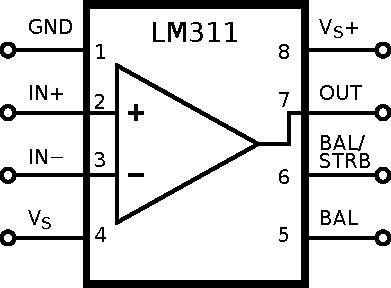
\includegraphics[width=0.240\textwidth]{../E04/latex/LM311.pdf}
  \end{center}
  \caption{Piedinatura dell'operazionale LM311.}
  \label{cir4:piedinatura_LM311}
\end{wrapfigure}

L'amplificatore operazionale LM311 ha uno slew rate molto elevato e lavora sull'ordine dei nanosecondi: rispetto agli $0.5$\si{\volt\per\micro\second} del $\mu$A741, lo slew rate particolarmente alto permette di confrontare più velocemente i segnali.
Il funzionamento in configurazione di open loop dell'integrato può essere schematizzato, semplificandolo, come un transistor BJT a collettore aperto, in cui il collettore del transistor rappresenta l'output dell'opamp e l'emettitore è collegato a comune (Figura \ref{cir4:open_collector}).
Se colleghiamo anche una resistenza $R$ fra una tensione arbitraria $V_C$, la funzione di output dell'operazionale assume la forma di

\begin{equation}
V_{out} = \bigg \{
\begin{array}{rl}
V_C & \mathrm{se} \quad V_+ < V_- \\
0 & \mathrm{se} \quad V_+ > V_- \\
\end{array}
\label{eq4:comparatore}
\end{equation}

dove $V_+$ e $V_-$ sono rispettivamente le tensioni all'ingresso non invertente ed invertente. Utilizzando la schematizzazione con il transistor, è come considerare la condizione di quest'ultimo nei seguenti stati

\begin{equation}
Q : \bigg \{
\begin{array}{rl}
\mathrm{interdizione} & \mathrm{se} \quad V_+ < V_- \\
\mathrm{saturazione} & \mathrm{se} \quad V_+ > V_- \\
\end{array}
\label{eq4:comparatore_Q}
\end{equation}

da cui è facile mostrare che la tensione di uscita è proprio (\ref{eq4:comparatore}).

\begin{figure}[ht]
        \centering
        \begin{subfigure}[c]{0.5\textwidth}
		\centering
		  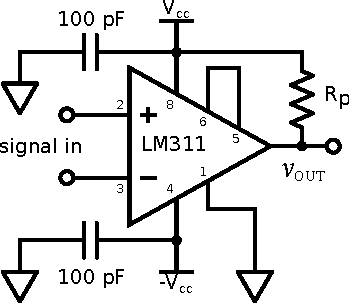
\includegraphics[height=4.3cm]{../E04/latex/c_comparatore.pdf}
		  \caption{Schema completo del comparatore utilizzato. La resistenza $R_p=\SI{9.98\pm0.01}{\kilo\ohm}$, come consigliato sul datasheet.}
		  \label{cir4:comparatore}
        \end{subfigure}%
    \quad
        \begin{subfigure}[c]{0.45\textwidth}
		\centering
		  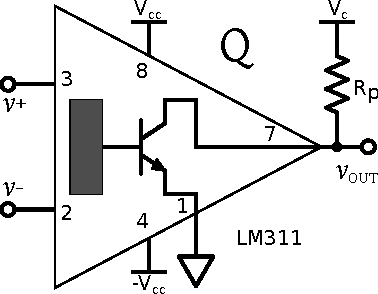
\includegraphics[height=4.3cm]{../E04/latex/c_LM311.pdf}
		  \caption{Schema semplificativo a collettore aperto dell'amplificatore operazionale LM311.}
		  \label{cir4:open_collector}
        \end{subfigure}
	\caption{}
\end{figure}

Quando Q è in saturazione la tensione di uscita (tensione di collettore) si porta circa alla tensione di emettitore, dunque a zero\footnote{In realtà la tensione di uscita risulterà qualche centinaio di \si{\milli\volt} sopra lo $0$, in quanto il transistor in saturazione ha una caduta di potenziale tra l'emettitore e il collettore.}.
Quando Q è interdetto, invece, il generatore di tensione che fornisce $V_C$ non eroga corrente (l'impedenza dell'oscilloscopio è \SI{1}{\Mohm}) e quindi non c'è caduta ai capi di $R$, dunque $V_{out}=V_C$.
È bene notare che la tensione di uscita è definita non dall'amplificatore ma dalla tensione $V_C$ e dalla presenza della resistenza $R$, che serve anche a limitare la corrente che scorre in Q in saturazione.

Possiamo pertanto confrontare le tensioni agli ingressi sfruttando il funzionamento di questo opamp.
Poniamo, ad esempio, l'ingresso invertente ad una tensione di soglia $V_{ref}$: se vale la (\ref{eq4:comparatore}), ponendo un segnale in alternata sull'ingresso non invertente, l'operazionale restituirà una $V_{out}$ nulla se $V_{in}<V_{ref}$, altrimenti $V_C$.
Valutiamo dunque il funzionamento del circuito ipotizzato, il cui schema circuitale è riportato in Figura \ref{cir4:comparatore}, ponendo $V_{C}=5$\si{\volt}.
Il grafico in Figura \ref{gr4:comparatore} mostra le tensioni in entrata e in uscita dal circuito.
\newpage
\begin{figure}[ht]
 \centering
   {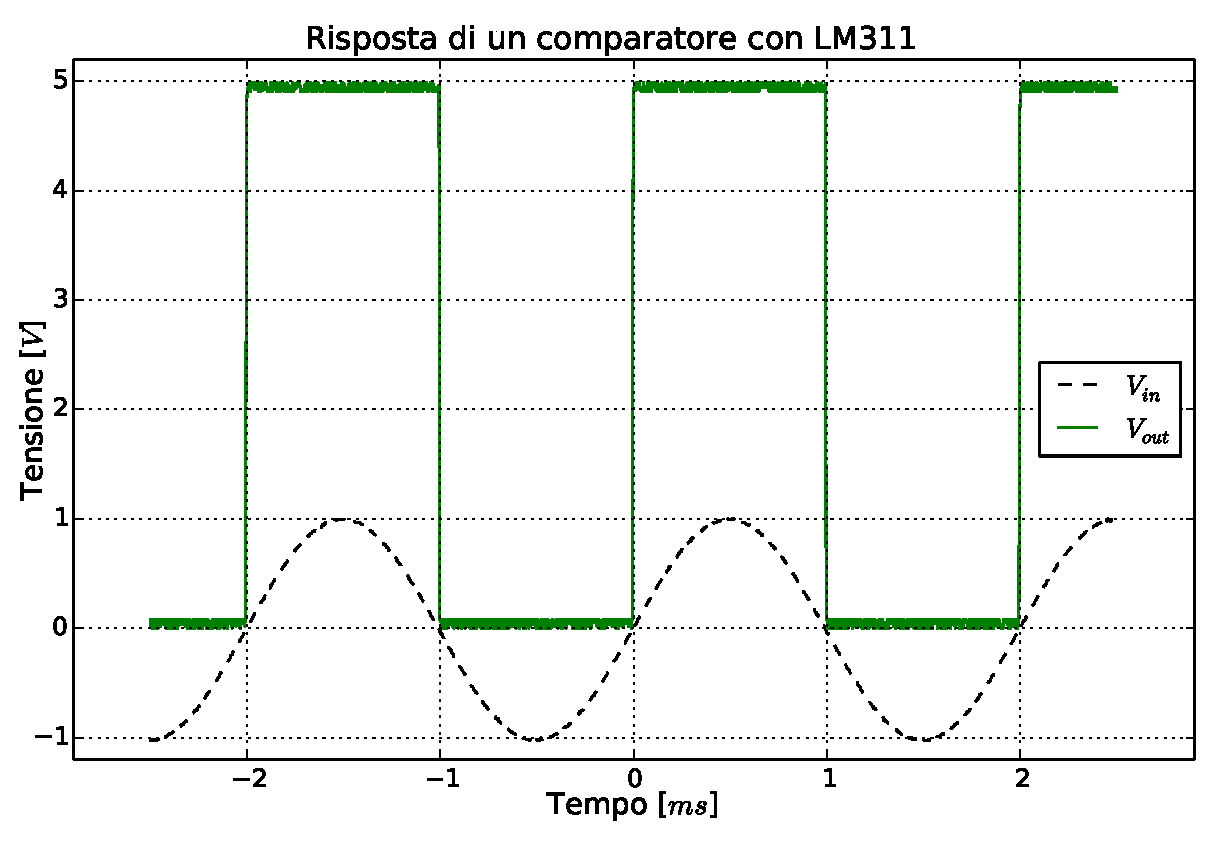
\includegraphics[width=14cm]{../E04/latex/comp.pdf}}
 \caption{Grafico della tensione in entrata (onda sinusoidale con $V_{pp}=2$ \si{\volt} e $f=500$\si{\hertz}, tratteggiata) e in uscita (verde) in funzione del tempo. Notiamo che l'uscita rispetta (\ref{eq4:comparatore}).}
 \label{gr4:comparatore}
\end{figure}

\subsection{Trigger di Schmitt non-invertente}

\begin{wrapfigure}[16]{r}{0.50\textwidth}
  \begin{center}
    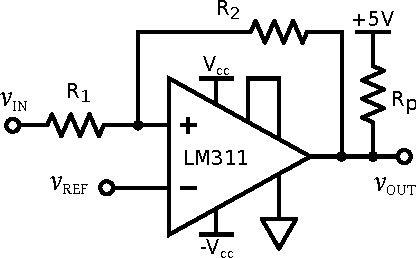
\includegraphics[width=0.320\textwidth]{../E04/latex/c_schmitt.pdf}
  \end{center}
  \caption{Schema del trigger di Schmitt. Le resistenze $R_1$ e $R_2$ sono state variate, mentre $R_p=\SI{9.98\pm0.01}{\kilo\ohm}$, come consigliato sul datasheet.}
  \label{cir4:schmitt}
\end{wrapfigure}

Quando nel segnale è presente un rumore è possibile che il valore di tensione restituito dal comparatore cambi più volte da $0$ a $V_{C}$.
Infatti, l'ampiezza in tensione del rumore può essere tale da passare sopra e sotto la tensione di soglia, invertendo la $V_{out}$ più volte, in accordo con (\ref{eq4:comparatore}).

Per ovviare a questo problema si sfrutta la retroazione positiva dell'amplificatore operazionale per riportare parte della $V_{out}$ sull'ingresso non invertente: ciò permette di creare un offset positivo sulla tensione all'ingresso non invertente quando $V_{in}>0$ e viceversa.
Quindi, durante il confronto del segnale con la tensione di riferimento, il segnale in entrata risulterà aumentato o diminuito di una certa quantità a seconda di $V_{out}$.

Valutiamo queste tensioni di soglia nel trigger di Schmitt non invertente (grafico in Figura \ref{cir4:schmitt}).
Per fare ciò cerchiamo la dipendenza di $V_{in}$ da $V_{out}$ e da $V^+$ (tensione all'ingresso non invertente). Utilizzando la legge di Kirchhoff sul nodo dell'ingresso non invertente
$$\frac{V_{in}-V^+}{R_1} + \frac{V_{out}-V^+}{R_2} = 0$$
da cui otteniamo
\begin{equation}
V_{in} = V^+ \frac{R_1+R_2}{R_2} - V_{out} \frac{R_1}{R_2}
\label{eq4:v_in_parte2}
\end{equation}
Dunque otteniamo i valori di soglia (che sono valori di $V_{in}$) ponendo la tensione $V^+=V^-=V_{ref}=0$, cioè il punto di tensione di inversione del comportamento del LM311 a collettore comune, e considerando i due valori possibili di $V_{out}$ dati dalla (\ref{eq4:comparatore}), cioè $V_{out}^{inf}=0$ e $V_{out}^{sup}=V_{C}=5$\si{\volt}:
$$V_{soglia}^{sup} = - V_{out}^{inf} \frac{R_1}{R_2} = 0 \qquad V_{soglia}^{inf} = - V_{out}^{sup} \frac{R_1}{R_2} = - (0.46 \pm 0.01) \si{\volt}$$
da cui è possibile definire la tensione di \textit{isteresi} (cioè la tensione massima in cui un segnale può oscillare attorno alla tensione di riferimento prima di ribaltare l'output del LM311)
$$V_{isteresi} = |\Delta V| = |V_{soglia}^{sup} - V_{soglia}^{inf}| = V_{out}^{sup} \frac{R_1}{R_2} = (0.46 \pm 0.01) \si{\volt}$$

I punti così calcolati sono visibili nel grafico di isteresi in Figura \ref{gr4:isteresi}.

Notiamo però che vi sono alcune incongruenze rispetto al grafico ideale di isteresi: le rette $V_{in}=V_{soglia}$ (per entrambe le soglie) in realtà non sono perpendicolari alle ascisse, e abbiamo ipotizzato che tale comportamento sia imputabile all'entrata dell'opamp in regione lineare, uscendo dalla saturazione.
Inoltre la tensione di uscita massima non è $5$ \si{\volt} perché, a differenza del comparatore in Figura \ref{cir4:comparatore}, la corrente quando Q è interdetto può passare attraverso il circuito di retroazione, provocando una caduta di potenziale sulla resistenza $R$.
Tale corrente dipende inoltre dalla tensione in entrata, dunque è spiegata la pendenza della retta $V_{out}^{sup}$.

Abbiamo infine provato ad inserire un offset all'ingresso invertente: ciò ha portato, come ci aspettavamo dalla relazione (\ref{eq4:v_in_parte2}) (si ricorda che $V^+=V_{ref}$), ad una traslazione del grafico in Figura \ref{gr4:isteresi} di un valore dato dall'offset impostato. Infine, durante l'esperienza, abbiamo anche variato $R_1$ per valutare diverse tensioni di isteresi.

\begin{figure}[ht]
 \centering
   {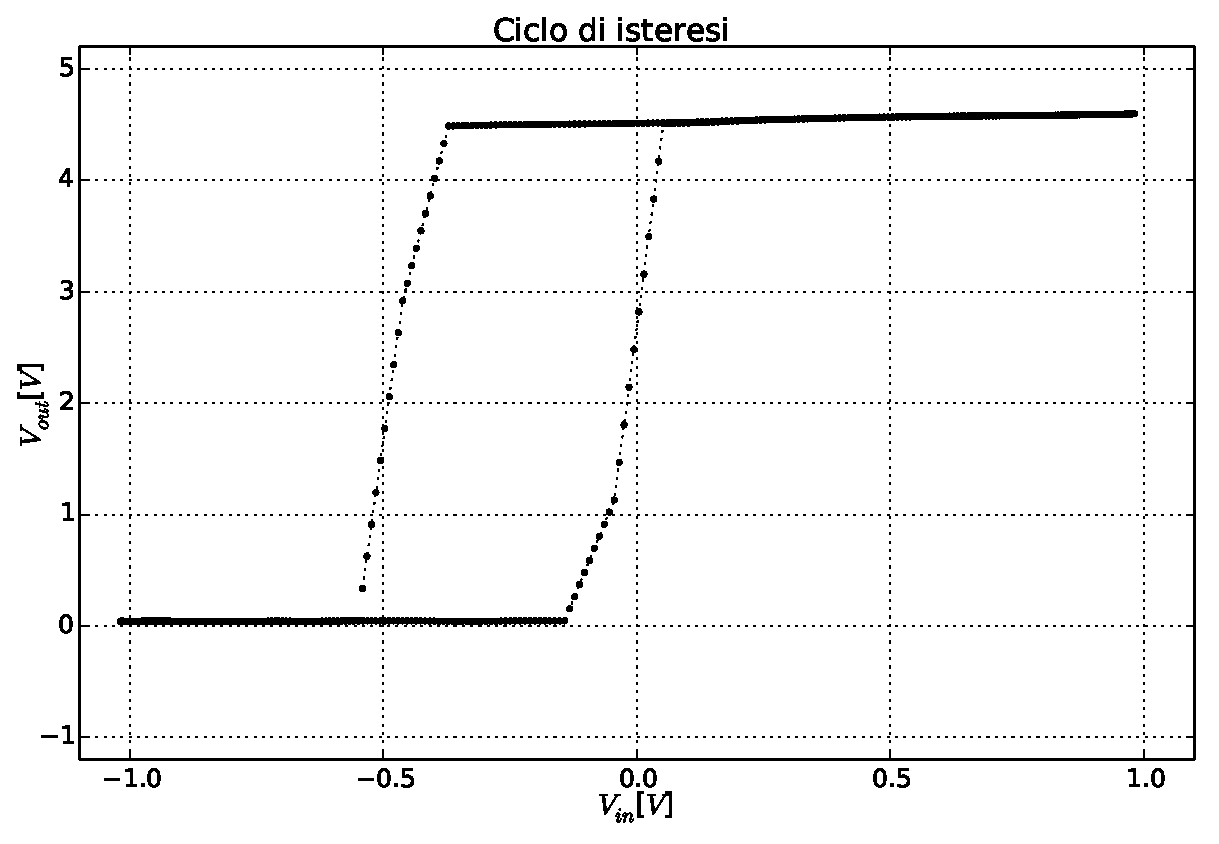
\includegraphics[width=14cm]{../E04/latex/XY.pdf}}
 \caption{Grafico dell'isteresi. Per questi dati le resistenze utilizzate sono $R_1=\SI{9.98(1)}{\kohm}$ e $R_2=\SI{99.6(1)}{\kohm}$. Le varie differenze rispetto al grafico ideale sono spiegate nel paragrafo.}
 \label{gr4:isteresi}
\end{figure}

\subsection{Oscillatore a rilassamento}

\begin{wrapfigure}[15]{r}{0.45\textwidth}
  \begin{center}
    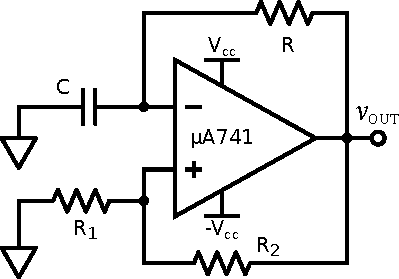
\includegraphics[width=0.30\textwidth]{../E04/latex/c_rilassamento.pdf}
  \end{center}
  \caption{Schema completo dell'oscillatore a rilassamento.}
  \label{cir4:oscillatore}
\end{wrapfigure}

In questa parte dell'esperienza studieremo il funzionamento di un oscillatore a rilassamento. Tale circuito sfrutta l'instabilità della retroazione positiva per generare un segnale oscillante con una frequenza determinata dai componenti stessi del circuito. In Figura \ref{cir4:oscillatore} è riportato lo schema circuitale. 

L'elemento circuitale fondamentale per il funzionamento dell'oscillatore a rilassamento è il condensatore C.  Sfruttando il trigger di Schmitt dato dalle resistenze $R_1$ ed $R_2$, la tensione di riferimento (cioè la tensione $V_+$ all'ingresso non invertente) cambia al cambiare di $V_{out}$ come segue
$$
V_{+} = \bigg \{
\begin{array}{rl}
\beta V_{cc} & \mathrm{se} \quad V_+ > V_- \quad \mathrm{ovvero} \quad V_{out}=V_{cc}\\
-\beta V_{cc} & \mathrm{se} \quad V_+ < V_- \quad \mathrm{ovvero} \quad V_{out}=-V_{cc}\\
\end{array}
$$
dove $\beta=\frac{R_1}{R_1+R_2}$ è dato dal partitore fra $R_1$ ed $R_2$.
Nel nostro caso, la capacità renderà la tensione $V_-$ all'ingresso invertente crescente (verso $V_{cc}$) quando $V_{out}=V_{cc}$ e decrescente nel caso opposto. Inoltre, $V_-$ invertirà il segno della derivata una volta raggiunta la tensione $\pm \beta V_{cc}$.

Infatti, supponiamo ad esempio che la tensione $V_-$ stia crescendo. Ciò significa, per quanto detto, che la tensione di riferimento è data dal trigger, cioè $V_+=\beta V_{cc}$. Dunque, una volta raggiunta e superata tale tensione il confronto fra le due invertirà la tensione di uscita e $V_-$ inizierà a decrescere fino a $-\beta V_{cc}$, per poi invertirsi di nuovo. Tale processo porta quindi ad una oscillazione a rilassamento, cioè verso una stabilizzazione a $\pm V_{cc}$ che però non può avvenire per la presenza del trigger. Il periodo di tale oscillazione può essere calcolato risolvendo il circuito.
%Per comodità a $t=0$ assumiamolo scarico e $V_{out}=+V_{sat}$. Ovviamente, per effetto della retroazione negativa, la tensione all'ingresso invertente tenderà ad aumentare ($V_{inv}$ è determinata da quanta carica è accumulata sul condensatore). Non appena $|V_{inv}|>|V_{ninv}|$, avremo uno switch della tensione in uscita, ovvero $+V_{sat} \rightarrow -V_{sat}$. Il condensatore inizierà dunque a scaricarsi. Successivamente avremo un altro switch della tensione in uscita e il ciclo si ripeterà. Il periodo di tale oscillazione può essere calcolato risolvendo il circuito.

A tal fine consideriamo la parte del circuito costituita dalla capacità C e dalla resistenza R per valutarne la risposta al gradino (cioè quando la tensione in uscita dal $\mu$741 passa da $-V_{cc}$ a $V_{cc}$), schematizzandolo come in Figura \ref{cir4:oscillatore_spi}, in quanto è il comportamento della capacità che ci interessa per il calcolo del periodo $T$.

\begin{wrapfigure}[18]{l}{0.22\textwidth}
  \begin{center}
    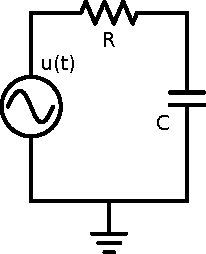
\includegraphics[width=0.20\textwidth]{../E04/latex/c_rilassamento_spi.pdf}
  \end{center}
  \caption{}
  \label{cir4:oscillatore_spi}
\end{wrapfigure}

Per la legge di Kirchhoff sulle correnti vale
$$\frac{u(t)V_{cc} - V(t)}{R} - C \frac{dV(t)}{dt} = 0$$
con $u(t)=1$ per $t>0$ e $V(t)=V_-$ la differenza di potenziale del condensatore. Quindi otteniamo
$$\frac{1}{V_{cc} - V(t)} \frac{dV(t)}{dt} = \frac{1}{RC}$$
L'equazione differenziale ha come soluzione
$$V(t)=V_{cc} - a \mathrm{e}^{-\frac{t}{RC}}$$
Per trovare la costante $a$ dobbiamo considerare il grafico in Figura \ref{gr4:osc10k} e impostare $V(t=0)=-\beta V_{cc}$. Quindi si ricava che
\begin{equation}
V(t)=V_{cc} - V_{cc} (1+ \beta) \mathrm{e}^{-\frac{t}{RC}}
\label{eq4:osc_vt}
\end{equation}
Sempre dal grafico sperimentale in Figura \ref{gr4:osc10k} è possibile imporre che $V(T/2)=\beta V_{cc}$. Imponendo l'uguaglianza di questa condizione con (\ref{eq4:osc_vt}) e svolgendo i calcoli il valore che si ottiene per il periodo è
\begin{equation}
T=2RCln\left(1+\frac{2R_1}{R_2}\right)
\label{eq4:periodo_osc}
\end{equation}  

Nel grafico in Figura \ref{gr4:osc10k} sono riportati i risultati ottenuti per valori di $R=\SI{9.99(1)}{\kohm}$. Come vediamo, carica e scarica del condensatore tendono a $\pm V_{sat}$.

Nella seguente tabella riportiamo i valori teorici e sperimentali di periodo dell'oscillatore a rilassamento.

\begin{center}
{\renewcommand{\arraystretch}{1.2}%
	\begin{tabular}{c|c|c}
    %\hline
	$R$ [\si{\kilo\ohm}] & $T_{exp}$ [\si{\milli\second}] & $T_{teo}$ [\si{\milli\second}]\\
    \hline
	$9.99\pm0.01 $ & $2.22\pm0.01$ & $2.19 \pm 0.03$\\
    \hline
	$99.93\pm0.01 $ & $22.2\pm0.1$ & $21.9 \pm 0.3$\\
    %\hline
	\end{tabular}
}
\end{center}

\begin{figure}[ht]
 \centering
   {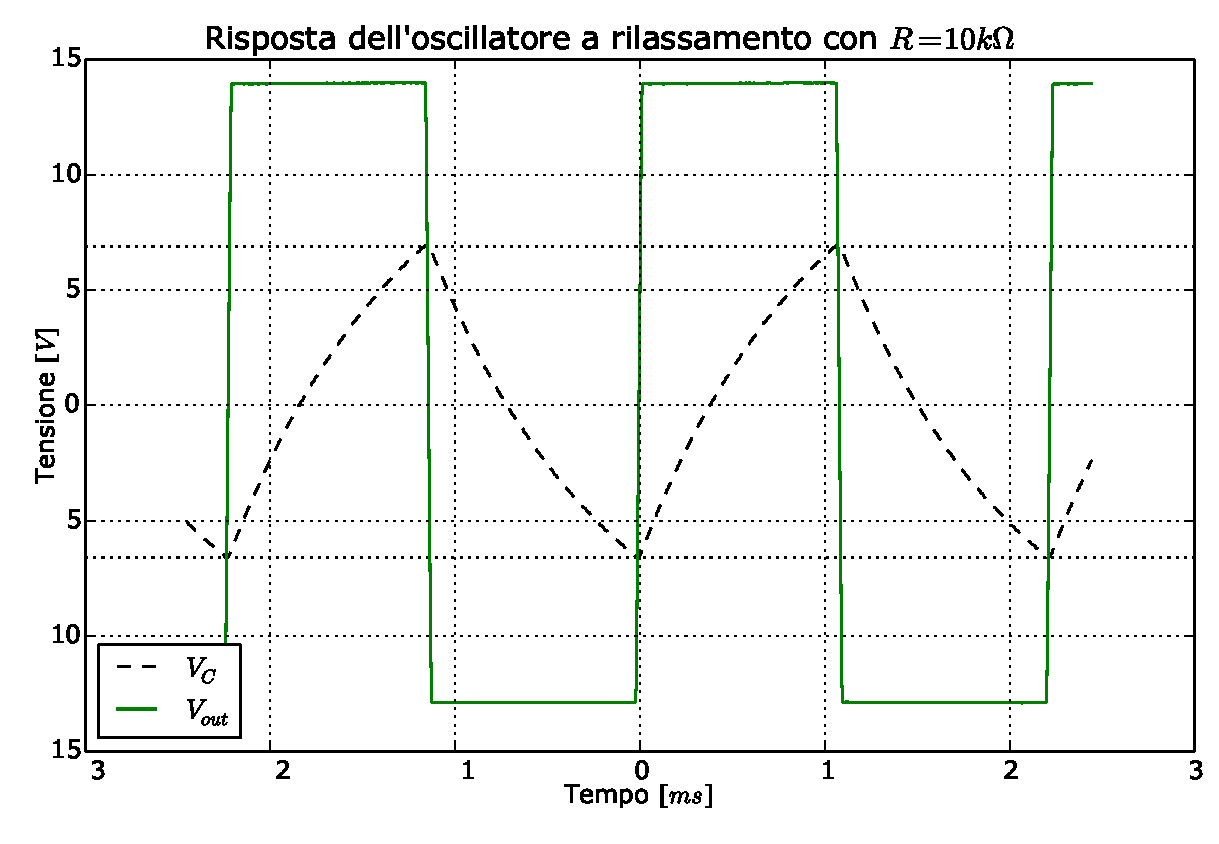
\includegraphics[width=14cm]{../E04/latex/osc10k.pdf}}
 \caption{Risposta del circuito oscillatore a rilassamento con $C=\SI{85.0(5)}{\nano\farad}$, $R=\SI{9.99(1)}{\kohm}$, $R_1= \SI{9.96(1)}{\kohm}$ e $R_2=\SI{9.98(1)}{\kohm}$.}
 \label{gr4:osc10k}
\end{figure}

\subsection{Interruttore crepuscolare}

Nell'ultima parte dell'esperienza abbiamo assemblato un interruttore crepuscolare, cioè un circuito elettronico che alimenta un carico (LED) in condizioni di bassa luminosità ambientale e interrompe l'alimentazione in condizioni di alta luminosità ambientale.

\begin{figure}[ht]
 \centering
   {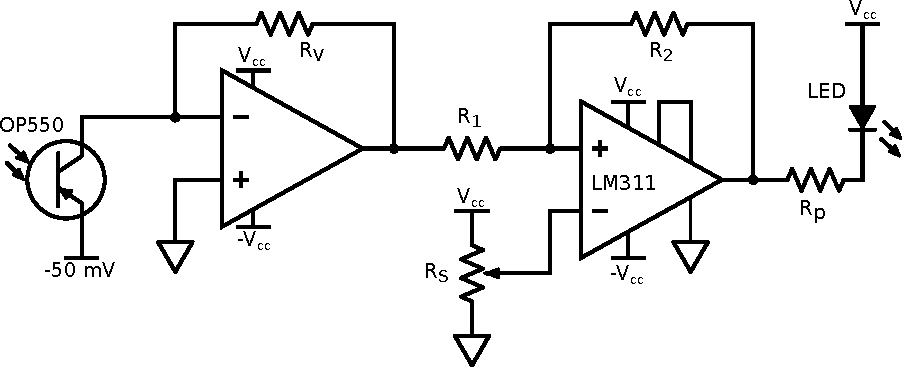
\includegraphics[width=13.5cm]{../E04/latex/c_crepuscolare.pdf}}
 \caption{Circuito dell'interruttore crepuscolare. Come vediamo chiaramente, la parte con l'op-amp $\mu$A741 è un semplice amplificatore in tensione ($R_F = \SI{1}{\Mohm}$) La seconda parte del circuito è un comparatore con isteresi, settata dal rapporto $R_1/R_2$ ($R_1 = \SI{50}{\kohm}$ e $R_2 = \SI{100}{\kohm}$). La tensione di riferimento deve essere scelta in modo da decidere con quanta luminosità si vuole che l'interruttore scatti. Per far ciò abbiamo usato un partitore utilizzando un trimmer ($R_S$) da \SI{10}{\kohm}. La resistenza di pull-up è stata scelta di  \SI{1}{\kohm}, così da avere una corrente sufficiente per far accendere il led.}
 \label{cir4:crepuscolare}
\end{figure}

Un circuito di questo tipo necessità di almeno due componenti: il sensore di luminosità (fototransistor OP550) che fornisce la variabile circuitale collegata alla luminosità ambientale e un blocco di comparazione che \textit{decide} se alimentare o meno il carico confrontando il segnale dato dal primo blocco con un segnale di riferimento.

Il componente principale del primo blocco è il fototransistor OP550 che agisce come una sorgente di corrente, generando una corrente dell'ordine del \si{\uA} se esposto alla luce.
Tale corrente è però difficilmente manipolabile, pertanto abbiamo deciso di utilizzare un convertitore corrente-tensione per trasformare e amplificare il segnale in modo tale da poter essere utilizzata come segnale di ingresso del secondo blocco.

\begin{figure}[ht]
 \centering
   {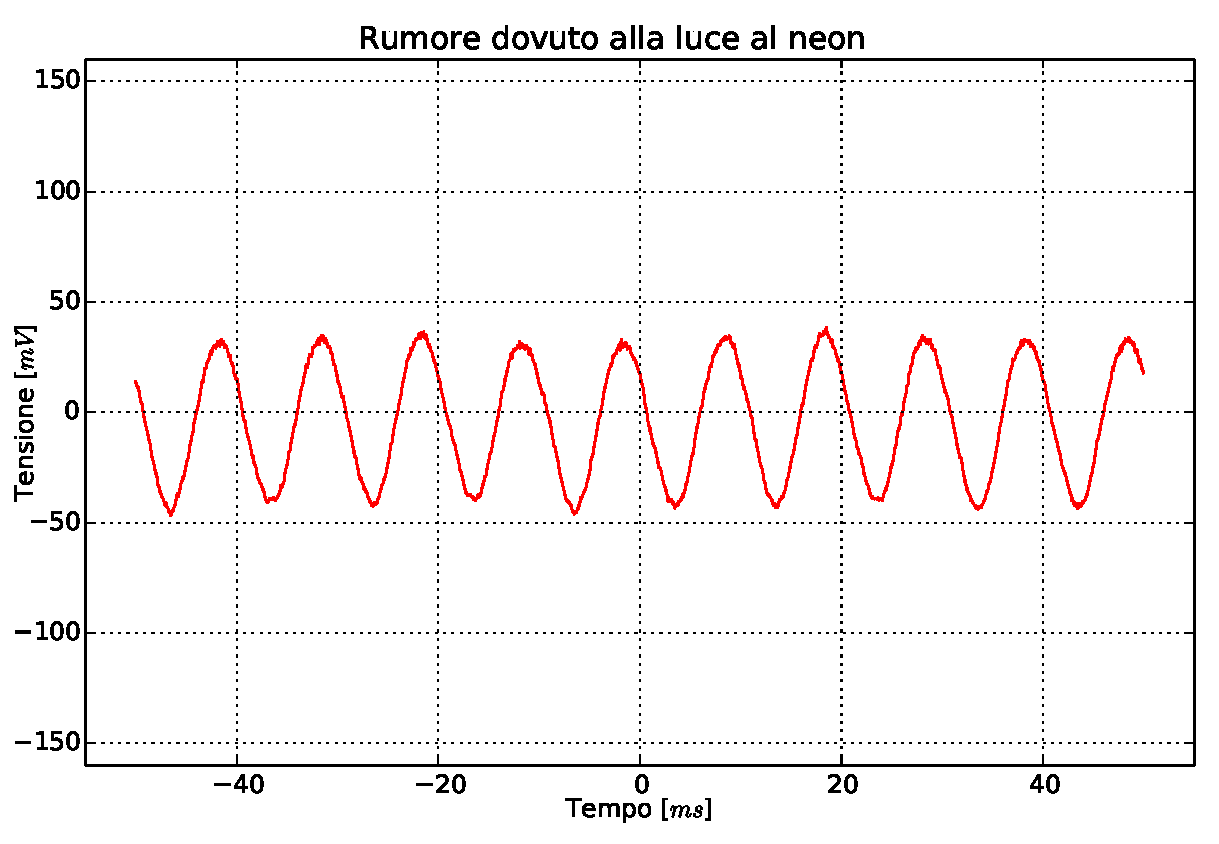
\includegraphics[width=14cm]{../E04/latex/neon.pdf}}
 \caption{Rumore ambientale determinato dalla luce delle lampade al neon del laboratorio incidente sul fototransistor e amplificato dall'opamp $\mu$A741. I dati sono stati ricavati separando i due blocchi del circuito e misurando la tensione all'uscita dell'opamp $\mu$A741.}
 \label{gr4:neon}
\end{figure}

Un convertitore corrente-tensione può essere implementato facilmente utilizzando un opamp $\mu$A741 in modalità di amplificatore invertente con retroazione negativa (vedi Figura \ref{cir4:crepuscolare}).
In questo modo, la tensione in uscita dell'opamp sarà legata alla corrente che attraversa il sensore dalla seguente equazione:

\begin{equation}
	V_{out} = R_F \,\, I_{OP550}
\end{equation}
dove $R_F$ è la resistenza posta sul ramo di retroazione (nel nostro caso $R_F = \SI{1}{\Mohm}$) e $I_{OP550}$ è il modulo della corrente passante nel fototransistor.

Il secondo blocco del circuito è invece composto da un opamp LM311 utilizzato come comparatore con isteresi (o trigger di Schmitt).
Sul ramo di retroazione e tra il terminale positivo e l'ingresso del segnale - che corrisponde all'uscita dell'opamp $\mu$A741 - sono state poste due resistenze per creare l'isteresi affinché eventuali rumori di fondo non disturbassero il funzionamento del circuito.
Nel nostro caso abbiamo utilizzato due resistenze $R_1 =$ \SI{5}{\kohm} e $R_2=$ \SI{100}{\kohm} in modo da avere un ampio margine di sicurezza.

Come si può notare dal grafico in Figura \ref{gr4:neon} il rumore ambientale dato dalle lampade al neon ha una forma d'onda sinusoidale di frequenza \SI{100}{\hertz} e ampiezza picco-picco \SI{80}{\mV}, pertanto sarebbe stata sufficiente un'isteresi di appena $\frac{V_{CC}}{100} \approx \SI{150}{\mV}$

Per impostare la tensione di soglia, invece, abbiamo creato un partitore collegando i due connettori esterni di un trimmer resistivo da \SI{10}{\kohm} a +\SI{15}{\V} e a comune, mentre abbiamo collegato il terminale centrale del trimmer all'ingresso invertente del LM311.
In questo modo potevamo scegliere la tensione di soglia girando semplicemente un cacciavite.

Infine abbiamo posto il carico da alimentare tra l'alimentazione positiva +\SI{15}{\V} e la resistenza di pull-up ($R_P=$ \SI{1}{\kohm}).

\subsection*{Conclusioni}

In questa esperienza abbiamo analizzato il funzionamento di circuiti comparatori, molto utili quando vogliamo confrontare due segnali ottenendo un semplice valore digitale (on-off).
Tuttavia, vista la sensibilità degli op-amp, abbiamo bisogno di un modo per evitare che il rumore influenzi le nostre comparazioni.
Per far questo abbiamo introdotto i circuiti con isteresi, ovvero con feedback-positivo.

Durante l'esperienza abbiamo anche costruito un oscillatore a rilassamento: la peculiarità di tale circuito è che esso oscilla tra $+V_{sat}$ e $-V_{sat}$ sebbene sia alimentato con tensioni continue.
La frequenza di tale oscillatore è univocamente determinata dai valori delle componenti circuitali.

È stato poi realizzato un interruttore crepuscolare.
Questi interruttori, contenenti un fototransistor, permettono ad esempio l'accensione (e spegnimento) delle luci stradali quando tramonta il sole.
Non volendo però che una semplice nuvola passeggera faccia accendere le luci, abbiamo introdotto la retroazione positiva per creare un'isteresi che renda il circuito insensibile al rumore (la nuvola).
